\chapter{Methodology}

\section{Data cleaning}

The original proposal did not allocate a great deal of time (2-3 weeks) to data cleaning (dealing with any problems the data may have and loading it into a format amenable to further processing) this turned out to be more difficult than expected and as such took significantly longer (4-5 weeks, including a visit to an MEG laboratory to learn more about the data acquisition methods and processing techniques - which proved invaluable).

Most of the data for the healthy control patients was in the same format of a text file consisting of one column per MEG channel and one column for the time vector with each sample being a separate row. However some of the subjects shared the format of the Alzheimer's and MCI patients in which each the data for each channel (and the time vector) were contained within separate folders. Furthermore, some of the subjects had their data in different units as all the data had been multiplied by a factor of $1\times10^{5}$ due to different conventions between the Spanish and English versions of Microsoft Excel which had been used to manipulate the raw data several years ago.

Eleven of the data files were corrupted. Initially it seemed that that it would be possible to still use these subjects - using interpolation to deal with the missing data and rejecting the epochs where the interpolation was used to remove any effect upon the final data. However this ended up being very time-consuming as some of the data had multiple corruptions and some was so corrupted that even attempted to partially load the data failed. Therefore as the eleven subjects represented less than 5\% of the total 233 healthy controls it was decided that it wasn't worth the time it would take to recover the data.

Almost all of the data had been downsampled at acquistion, however for reasons that remain unknown, three uncorrupted subjects and one of the corrupted ones had not been downsampled. As the desired sampling rate was known however, it was easy to downsample these subjects using the \texttt{decimate} function in MATLAB, this automatically filters the data first to satisfy the Nyquist criterion and avoid aliasing.

The \textit{Nyquist criterion} in this context refers to the requirement that the highest frequency contained in the signal is less than half of the sampling rate. If this is not the case then \textit{aliasing} will occur in which the frequency of the sampled signal does not match the frequency of the original continuous signal. This loss of information means that accurate reconstruction of the original signal is impossible. Thus prior to downsampling (reducing the sample rate), the signal is first passed through a low-pass filter with a threshold at the Nyquist frequency ($\frac{1}{2}$ of the new downsampled sampling rate) so that aliasing does not occur. \cite{Smith1999} 
It was decided to use the FieldTrip MATLAB library\cite{Oostenveld2011} designed for EEG/MEG analysis. This would make the artefact rejection easier to perform in a more rigorous and standardised manner. Unfortunately the FieldTrip library expected the data in the format output by the original MEG machine and not the format in which we had recieved the data. After many attempts to load the data it appeared it would not be successful and so we produced our own artefact rejection scripts in MATLAB. This proved to be unnecessary as following a discussion with the Cognitive and Computational Neuroscience group at the Centro de Tecnolog\`{i}a Biom\'{e}dica (CTB), Madrid we discovered that it was possible to 'trick' Fieldtrip into loading the data provided one could provide a data header file with correct sensor information from an actual MEG machine. As the group could provide us with such a file we were then able to successfully load the data into FieldTrip and thus use it for the artefact rejection and signal processing.

The age of the subjects (and MMSE scores for the diseased patients) were stored across various different Excel spreadsheets. As these had been compiled by hand there were some typos in the filenames and differing conventions that made it impossible to fully automate the process of extracting the data into MATLAB. However it was possible to semi-automate it such that only the filenames that didn't match an entry in the spreadsheet required further inspection, reducing the number of files to check from 220 to around 40 and thus significantly reducing the time required.

\section{Artefact Rejection}

The artefact rejection process was performed in FieldTrip as mentioned previously. It is performed by computing the z-score for each point in time for each channel:

\begin{equation} z_{\textrm{ch, t}} = \frac{x_{\textrm{ch, t}} - \mu_{\textrm{ch}} }{\sigma_{\textrm{ch}}} \end{equation}

where $\mu_{\textrm{ch}}$ is the mean of the channel signal and $\sigma_{\textrm{ch}}$ is the standard deviation of the channel signal whilst $x_{\textrm{ch, t}}$ is the value of the signal in a certain channel at a certain time. 

The z-score is accumulated across all channels:

\begin{equation} zsum_t = \sum\limits^{148}_{ch=1} = \frac{z_{\textrm{ch, t}}}{\sqrt{148}} \end{equation}

where the number of channels is 148. This accumulated z-score value is compared to a threshold set by the user and if it exceeds the threshold then that epoch is rejected across all channels.


\begin{figure}[h!]
  \centering
    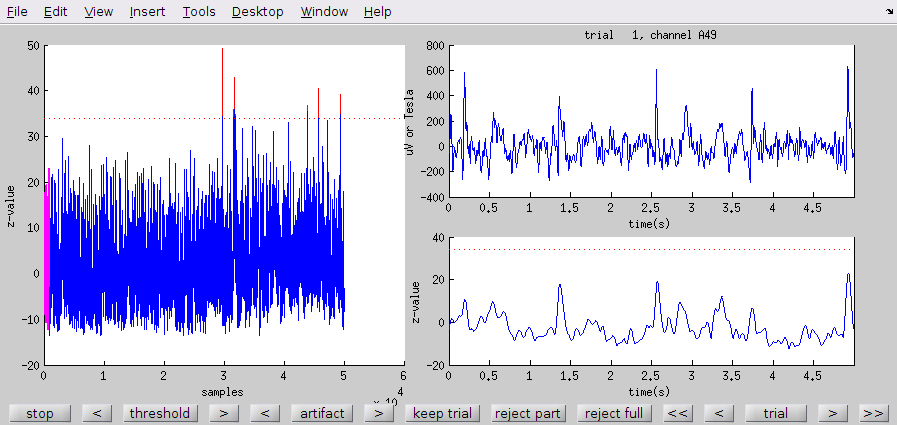
\includegraphics[width=\textwidth]{ftartefactgui.png}
    \caption{The artefact rejection GUI from FieldTrip.}
    \label{fig:ftartefactgui}
\end{figure}



Although it is possible to automate the entire process by setting a single threshold the differing noise levels between subjects meant that setting the same threshold for each subject resulted in extremely poor results. Therefore it was conducted using the manual Graphical User Interface (GUI) as shown in Figure \ref{fig:ftartefactgui}. This was quite a time-consuming process and took perhaps eight hours of solid work to process all the signals. However this approach which thresholds against the accumulated z-score was still much faster than inspecting each epoch for each channel for each patient. As there was an average of 60 5-second epochs per subject with 148 MEG channels and 278 subjects (combined total of healthy, MCI and AD) and so traditional visual inspection would have taken far too long as it would require the inspection of almost 2.5 million individual epochs.


\section{Filtering and Feature Extraction}

When the data was loaded into FieldTrip an 560th order Finite Impulse Response (FIR) filter with a Hamming window and a bandpass of 1.5 to 40Hz was applied as used by previous groups.\cite{Gomez2013}. The filter was applied to the whole signal rather than to each epoch separately to minimise edge effects (so the edge effects just occur at the first and last epochs, which can be discarded). The power spectral densities for each 5-second epoch were then obtained via Welch's method\cite{Welch1967} favoured for its noise reduction properties. See Figure \ref{fig:spectra} for an example PSD obtained from the dataset.


\begin{figure}[h!]
  \centering
    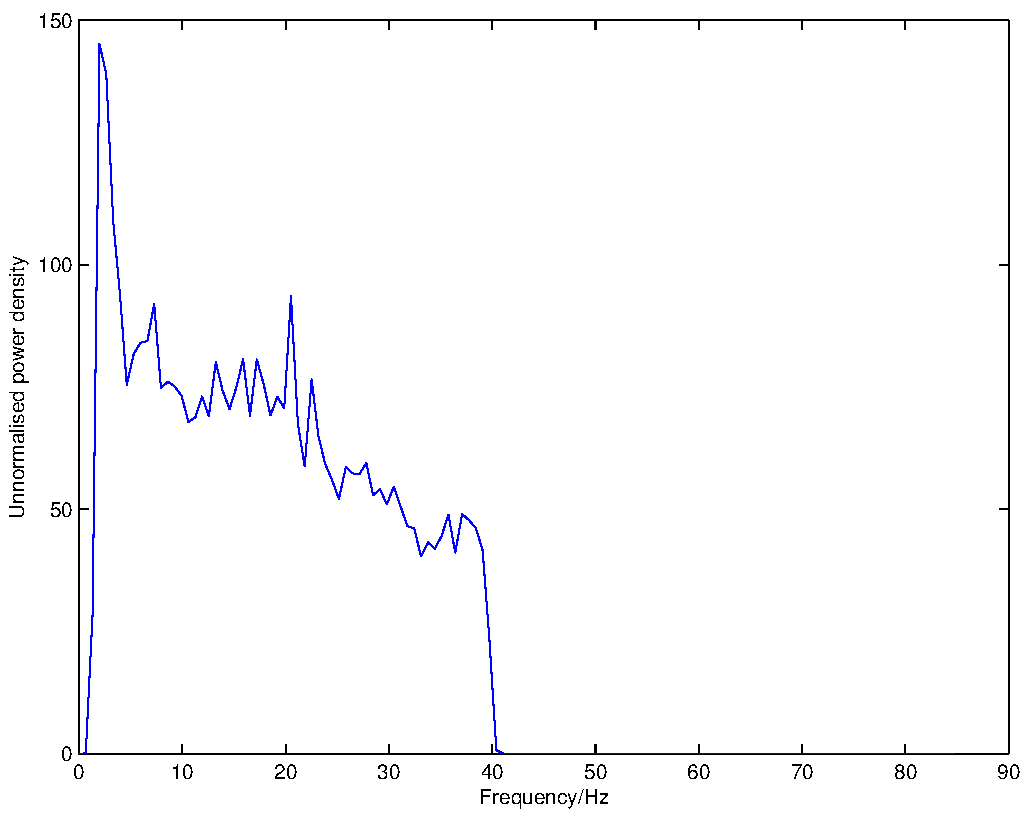
\includegraphics[width=0.8\textwidth]{postfilterexamplespectra.pdf}
    \caption{An example PSD taken from the data. Notice the sharp decline in power at 1.5 and 40 Hz due to the bandpass filter.}
    \label{fig:spectra}
\end{figure}

The relative powers were then calculated for each spectral band of interest (the conventional frequency bands associated with neural oscillations): delta (1.5-4 Hz), theta (4-8 Hz), alpha (8-13 Hz), the beta band was split into two sections - beta1 (13-19 Hz) and beta2 (19-30 Hz). The final band of interest is gamma (30-40 Hz). These are the same selection of bands used by previous groups. \cite{Gomez2013}. 

The relative powers are calculated by normalising the power spectral density (PSD) by the power contained in the total bandpass\cite{Escudero2013}:

\begin{equation} \textrm{PSD}_n(f)=\frac{\textrm{PSD}(f)}{\sum\limits^{40 \textrm{Hz}}_{f=1.5\textrm{Hz}} \textrm{PSD}(f) }   \end{equation}

and then computing the relative powers for each band from this normalised PSD:

\begin{equation} RP = \sum\limits^{f_{\textrm{high}}}_{f=f_{\textrm{low}}} PSD_n (f) \end{equation}

where $f_{\textrm{high}}$ and $f_{\textrm{low}}$ are the high and low cut-offs for the band respectively.

The relative powers were averaged over all accepted epochs and the channels were averaged into five brain regions (Central, Anterior, Left Lateral, Posterior, Right Lateral) shown in Figure \ref{fig:sensorareas}


\begin{figure}[h!]
  \centering
    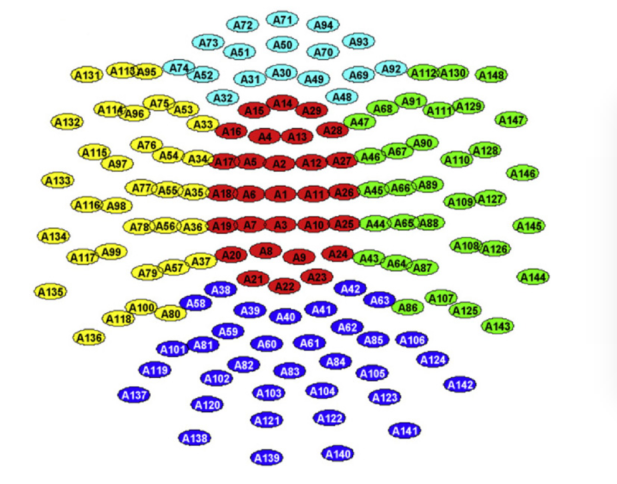
\includegraphics[width=0.8\textwidth]{sensorareas2.png}
    \caption{The division of the MEG channels into regions: Anterior (cyan), Central (red), Left Lateral (yellow), Right Lateral (green) and Posterior (blue) \cite{Escudero2013}}
    \label{fig:sensorareas}
\end{figure}

For some of the visualisations these regions were averaged over to reduce the number of features and thus the dimensionality of the data. This will be explicitly stated when the relevant visualisations are discussed. Averaging over the regions (i.e. averaging the relative powers over all channels) was also performed in previous studies \cite{Gomez2013} so it is reasonable to assume that there was not too much information lost.


\section{Model Fitting}

The features were fit with a multiple linear regression model:
\begin{equation} y = b_0 + b_1 x_1 + b_2 x_2 \cdots + b_{30} x_{30} \end{equation}
where $y$ is the dependent variable, the age of the subject, and $x_i$ are the explanatory variables (the relative powers of the different spectral bands in the different regions). The $b_i$ values are the regression coefficients, including the coefficient of the bias column of ones which was added to the feature vector in order to obtain the y-intercept of the fit.

The final model was obtained by a form of weighted model averaging. Tenfold cross-validation was used to obtain ten different models (i.e. ten sets of regression coefficients). Tenfold cross-validation involves partitioning the data into ten sets and training the model on 9 whilst using the remaining one as the test set, for all ten combinations. This prevents unrealistically optimistic error reports due to using the training data as a test set and thus provides a reasonable expectation of how well the model will generalise to unseen data. Furthermore, it is a natural means to obtain a number of models which can be used in model averaging to improve performance.

The model averaging was performed by calculating the weighted average of the regression coefficients from each model, weighted by the reciprocal of the root mean squared error (RMSE) value of each model:

\begin{equation} \vec{b}_{avg} = \frac{\sum\limits_{i=1}^{10} \vec{w}_i \vec{b}_i }{ \sum\limits_{i=1}^{10} \vec{w}_i}\end{equation}

where $\vec{w}_i = \frac{1}{\textrm{RMSE}_i}$.

Bootstrapping (i.e. sampling with replacement) \cite{Witten2011} was used to obtain an estimate of the RMSE of the averaged model on the Alzheimer's and MCI datasets. The estimates used 1000 bootstrap iterations which allows for an accurate estimation of the standard deviation of the sample distribution of the RMSE statistic (i.e. the standard error of the true distribution of the RMSE statistic). Each bootstrap set contained as many data points as in the set as a whole (so the Alzheimer's bootstraps each consisted of 39 samples and the MCI ones of 18 samples) - this is known as the \textit{0.632 bootstrap} as each set will contain 63.2\% of the unique data samples on average. It is the most common bootstrapping method. \cite{Witten2011}
\begin{table}[h!]
\begin{center}
\begin{tabular}[h!]{|c|c|c|}
\hline
Dataset & RMSE Mean & RMSE Sample standard error \\
\hline
Healthy & 14.86 & 2.68 \\
\hline
MCI & 22.72 & 3.03 \\
\hline
AD & 26.93 & 2.65\\
\hline
\end{tabular}
\caption{The RMSE values obtained on the model from each of the datasets.}
\label{tab:rmsevals}
\end{center}
\end{table}

The residuals of the model fit demonstrate the difference between the predicted age of the model and the subject's actual age. These were plotted against the subjects MMSE scores in Figure \ref{fig:cogscorecorrel} (MMSE data only available for Alzheimer's and MCI patients, not healthy subjects).

\begin{figure}[h!]
  \centering
    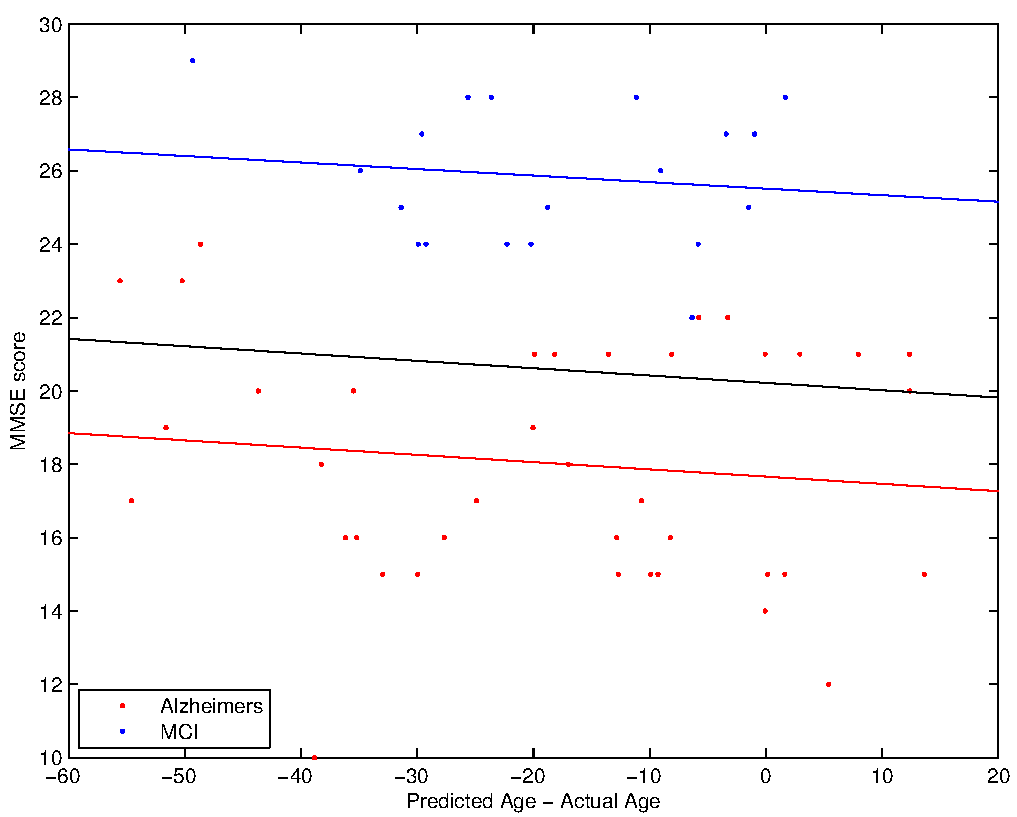
\includegraphics[width=\textwidth]{cogscorecorrel.pdf}
    \caption{The MMSE score plotted against the residuals of the model, the lines of best fit are plotted for each group. The black line is the line of best fit for the two groups combined. The correlations are very weak: the $r^2$ statistics are 0.0146 for the AD group (blue), 0.0168 for the MCI group (red) and 0.0060 for the two groups combined (black)}
    \label{fig:cogscorecorel}
\end{figure}





\section{Data visualisation}

As the data consisted of 30 features (6 spectral bands $\times$ 5 sensor regions) it cannot easily be visualised in a two-dimensional space amenable for printing, however it is possible to project the to a lower dimensional space or to display the relationships between feature values in a different manner (in the case of the parallel co-ordinate plot).


\subsection{t-Distributed Stochastic Neighbour Embedding}

t-Distributed Stochastic Neighbour Embedding (t-SNE)\cite{Maaten2008} is a data visualisation technique that maps the original high dimensional space of the data to a lower dimensional space (usually two-dimensional by default) to allow the data to be visualised. For example, one may produce a scatter plot of the high-dimensional data once it has been projected into two-dimensions. t-SNE reduced the dimensionality of the data whilst trying to retain as much of the high-dimensional structure as possible.

 It does this by computing a similarity metric between each pair of points by centering a Gaussian on one of the points in the high-dimensional space and using the probability density as the similarity metric. A Student's t-distribution with a single degree of freedom is used in the lower dimensional space in order to provide a more convenient cost function and avoid the \textit{crowding problem} due to insufficient area in the low dimensional space to accommodate all the nearby data points whilst retaining an accurate model of small distances. The differences between the similarity metrics in the high-dimensional space and the low-dimensional map are minimised as measured by the Kullbeck-Liebler divergence.\cite{Maaten2008}

 Thus t-SNE has the advantages that it is able to faithfully retain both the small-scale local structure of the high-dimensional data and the long-range global structure combined with a cost function that is easier to compute than traditional SNE which used Gaussian distributions in both the high and low dimensional spaces.\cite{Maaten2008}

 For example, see the t-SNE plot for the MNIST dataset of handwritten digits shown in Figure \ref{fig:mnisttsne}. The different classes are clearly separable which shows that classification of the digits should be possible from the data given.


\begin{figure}[h!]
  \centering
    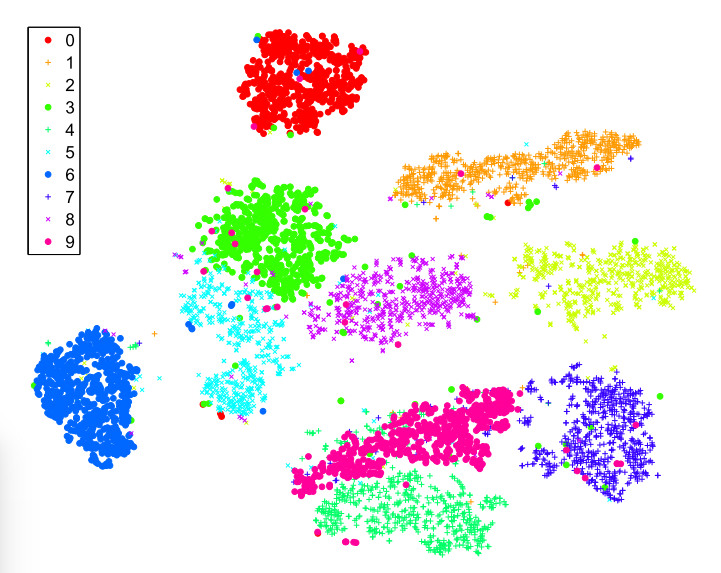
\includegraphics[width=\textwidth]{mnisttsne.png}
    \caption{The t-SNE visualisation of 6000 handwritten digits from the MNIST data set.\cite{Maaten2008} Note that the classes are clearly separable.}
    \label{fig:mnisttsne}
\end{figure}


t-SNE plots of each class (healthy, MCI or AD) with the samples separated by age were produced to see if within a disease group the age could be distinguished. This resulted in Figures \ref{htsneplot}, \ref{mcitsneplot} and \ref{alztsneplot}. As can be seen in the plots the different age groups were not separable and so it does not seem as though the relative powers gave much information about age when excluding the effects of disease.


\begin{figure}[h!]
  \centering
    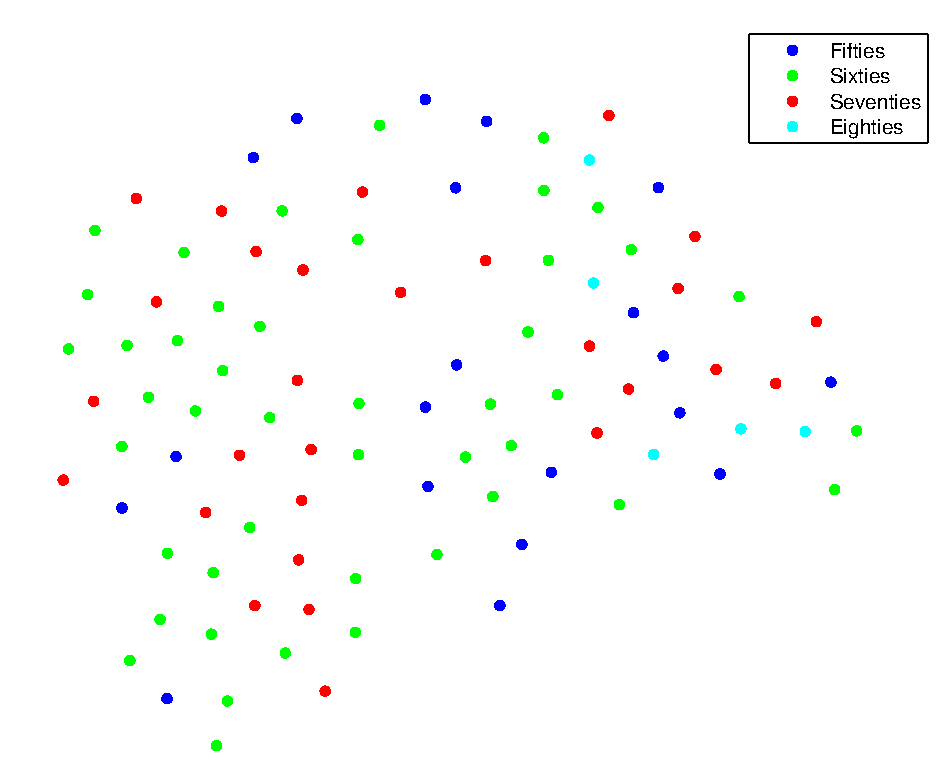
\includegraphics[width=\textwidth]{htsneplot.pdf}
    \caption{The t-SNE visualisation of the healthy subjects, divided into age groups. Note that the groups are not separable.}
    \label{fig:htsneplot}
\end{figure}


\begin{figure}[h!]
  \centering
    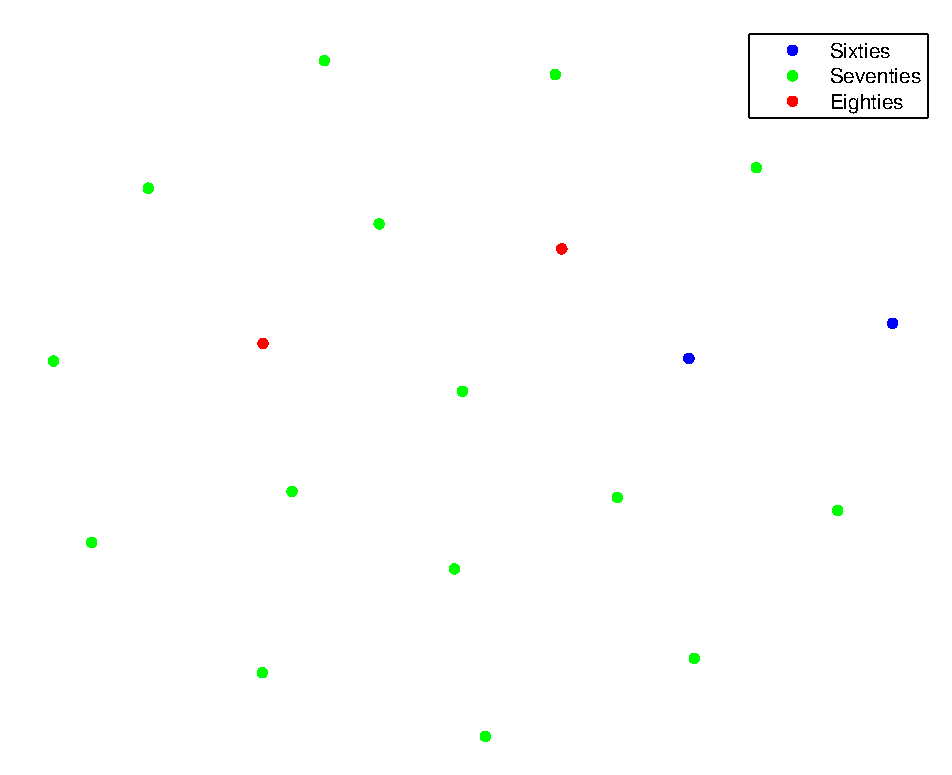
\includegraphics[width=\textwidth]{mcitsneplot.pdf}
    \caption{The t-SNE visualisation of the MCI patients, divided into age groups. Note that the groups are not separable.}
    \label{fig:mcitsneplot}
\end{figure}


\begin{figure}[h!]
  \centering
    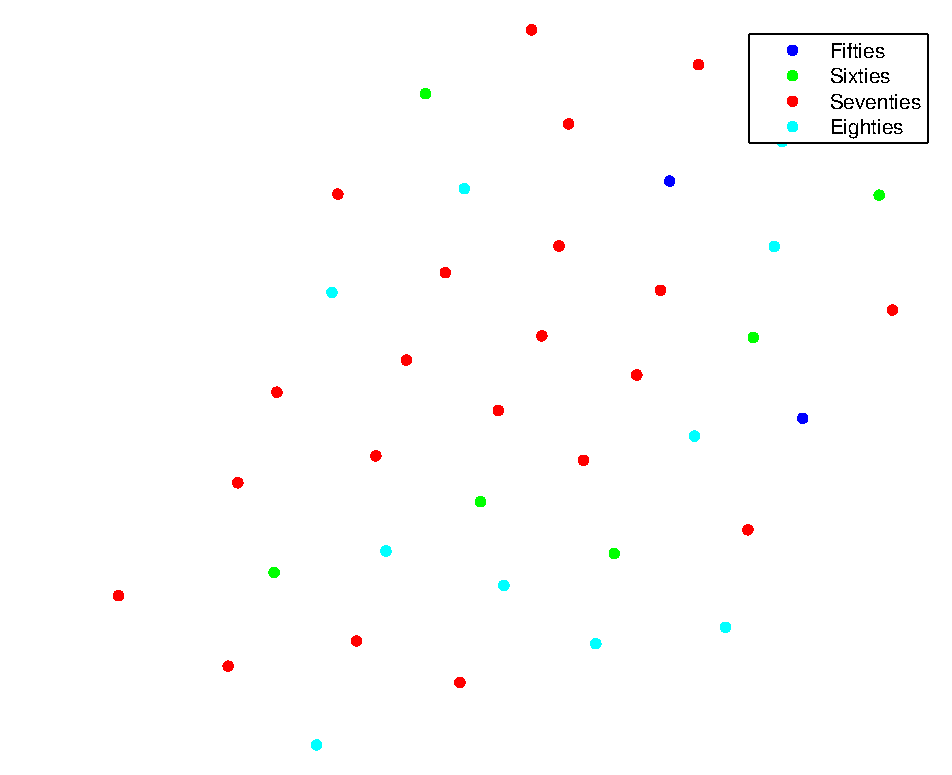
\includegraphics[width=\textwidth]{alztsneplot.pdf}
    \caption{The t-SNE visualisation of the AD patients, divided into age groups. Note that the groups are not separable.}
    \label{fig:alztsneplot}
\end{figure}


The total dataset was plotted to see if it was possible to distinguish between the healthy, MCI and AD subjects (see Figure \ref{fig:tottsneplot}). It did not appear to be the case, however it is possible that the effect of differing age might cause overlap between the disease groups simply due to the age difference between some members (e.g. if the young AD subjects overlapped with the old healthy ones then they would not appear as separable but it would still be possible to distinguish the classes). To take this into account we also plotted all the classes just for a single age group (subjects aged 70-79) as shown in Figure \ref{fig:seventiestsneplot}. The fact that the classes were still not separable was bad as it meant that classification would be at best difficult, if not impossible, using the given data.


\begin{figure}[h!]
  \centering
    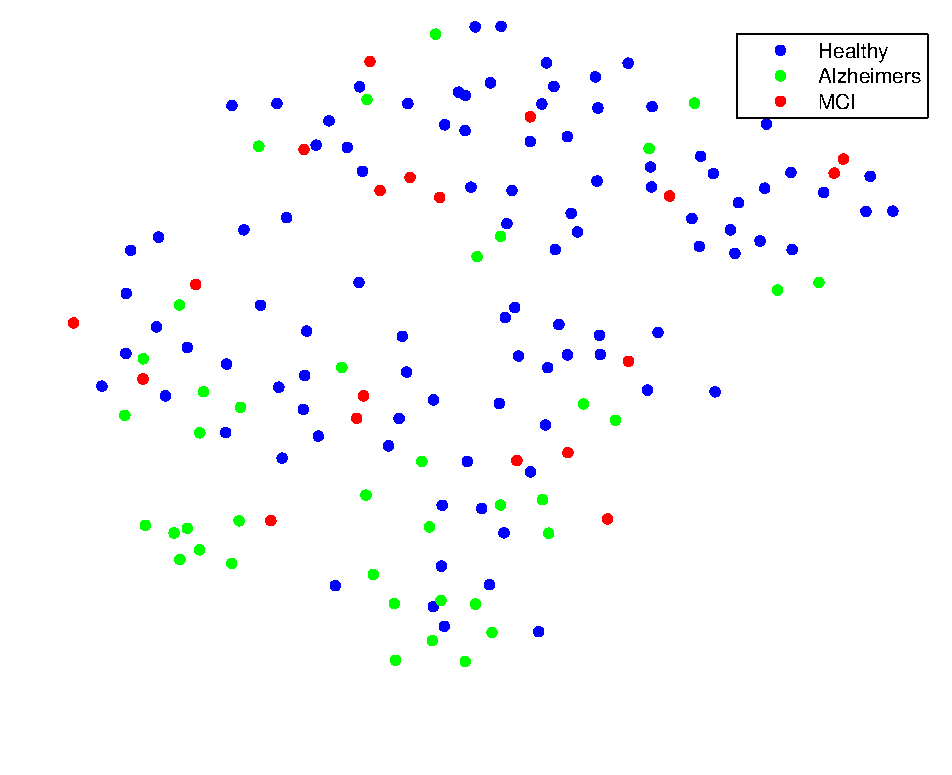
\includegraphics[width=\textwidth]{tottsneplot.pdf}
    \caption{The t-SNE visualisation of all the groups. Note that the groups are not separable but this could be due to the effect of age.}
    \label{fig:tottsneplot}
\end{figure}


\begin{figure}[h!]
  \centering
    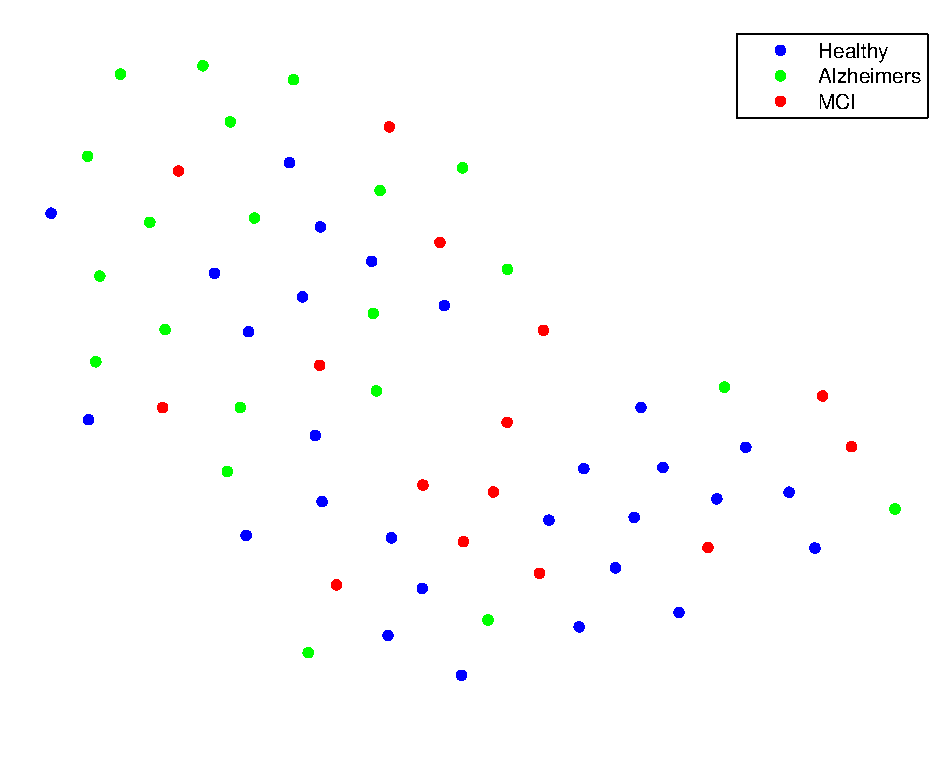
\includegraphics[width=\textwidth]{seventiestsneplot.pdf}
    \caption{The t-SNE visualisation of the all the groups, only subjects aged 70-79. Note that the groups are not separable. This implies classification will be difficult if not impossible.}
    \label{fig:seventiestsneplot}
\end{figure}



\subsection{Principal Components Analysis}

In contrast to the non-linear dimensionality reduction of t-SNE, Principal Components Analysis (PCA) is a linear projection of the data onto lower dimensional axes oriented such that the maximal amount of variation of the high dimensional data is preserved. \cite{Bushati2011} It is computed from the principal eigenvectors of the covariance matrix of the data. However PCA prioritises maintaining large-scale global structure over local structure in the data and so although the distances between distant points are well depicted, information contained within the distances between local points may be lost as the distances between proximal points are not as well depicted.

An advantage to PCA is that it still has defined axes whereas t-SNE just displays the pairwise similarity between points via the separation between them. Although the PCA axes may not always be physically meaningful (as it is just a linear combination of the original features) it can be useful to know which of the original features are responsible for most of the variance in the data and this information can be extracted from the principal components.

For the PCA plots the data used was a reduced feature set of six features: the spectral bands averaged over all brain regions. This was done such that the projections of the original axes could also be placed onto the plot so that it was possible to easily see which features contributed the most to the principal components - if this had been done with the full set of 30 features the plot would have been much too crowded. The plots are two-dimensional scatter plots using the first two principle components (i.e. the two that explain the most variance) because three-dimensional plots are difficult to clearly interpret when printed as one cannot rotate them so they may be misleading.

Plots were produced for the healthy dataset across all age groups as shown in Figure \ref{fig:pcahealthyplot} and for all classes across all age groups as shown in Figure \ref{fig:pcatotalplot}. These were not separable and as their t-SNE plots were not separable either and t-SNE is generally believed to be better at retaining the inherent high dimensional structure of the data\cite{Bushati2011} there seemed little benefit in including the other plots which just had the same result.

\begin{figure}[h!]
  \centering
    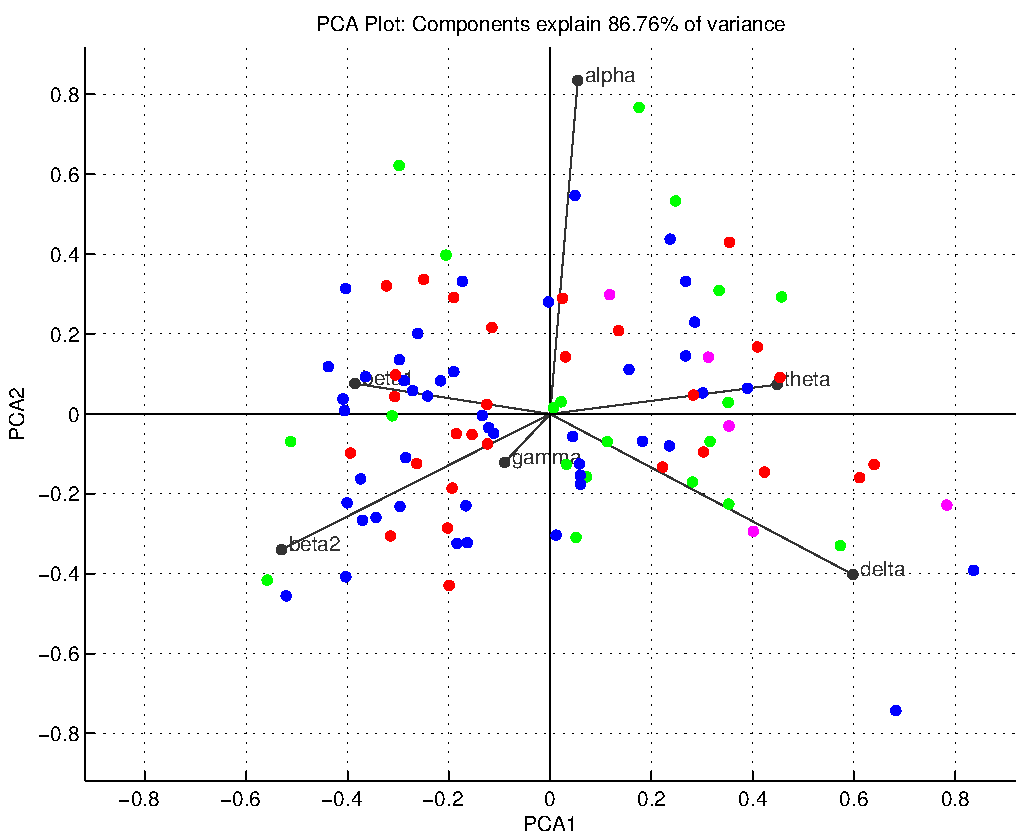
\includegraphics[width=\textwidth]{pcahealthyplot.pdf}
    \caption{The PCA projection of the healthy dataset, the two principal components explained 86.76\% of the data. The age groups following age groups were plotted: 50-59 (green), 60-69 (blue), 70-79 (red), 80-89 (magenta). Note that the groups are not separable.}
    \label{fig:pcahealthyplot}
\end{figure}

\begin{figure}[h!]
  \centering
    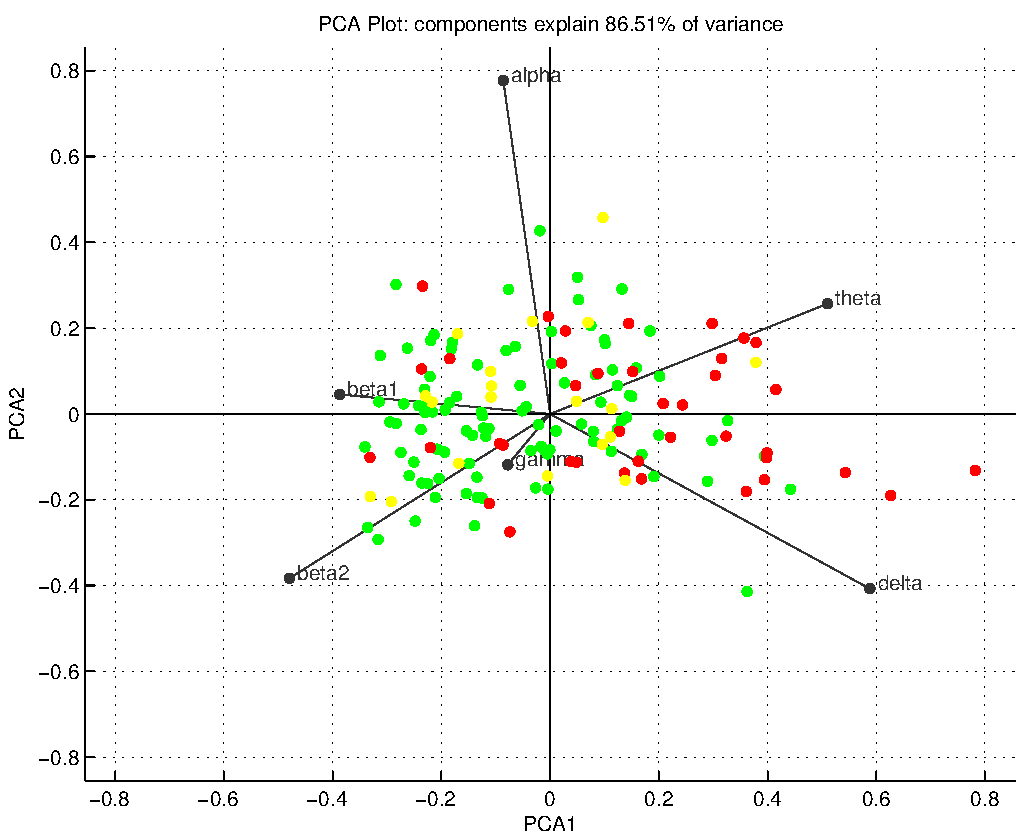
\includegraphics[width=\textwidth]{pcatotalplot.pdf}
    \caption{The PCA projection of the total dataset, the two principal components explained 86.51\% of the data. The classes are displayed as follows: Healthy (green), MCI (yellow), Alzheimer's Disease (red). Note that the groups are not separable.}
    \label{fig:pcatotalplot}
\end{figure}



\subsection{Parallel Coordinates plots}

A popular method to investigate the relationships between variables is the Parallel Coordinates Plot (PCP). It can also be used to examine the differences between classes and has had many applications ranging from optimising manufacturing to economic modelling \cite{Inselberg1997}.

The PCPs were produced using the reduced feature set (the same as used for the PCA plots) so that the axes could be reasonably spaced.

In the PCP each polyline represents a datapoint and it intercepts the axes at the value it has in the dimension represented by that axis. Therefore parallel lines between axes indicate a positive correlation between them, where crossing of lines in an X-shape indicates a negative correlation and random crossing indicates little or no relation.\cite{Inselberg1997}

\begin{figure}[h!]
  \centering
    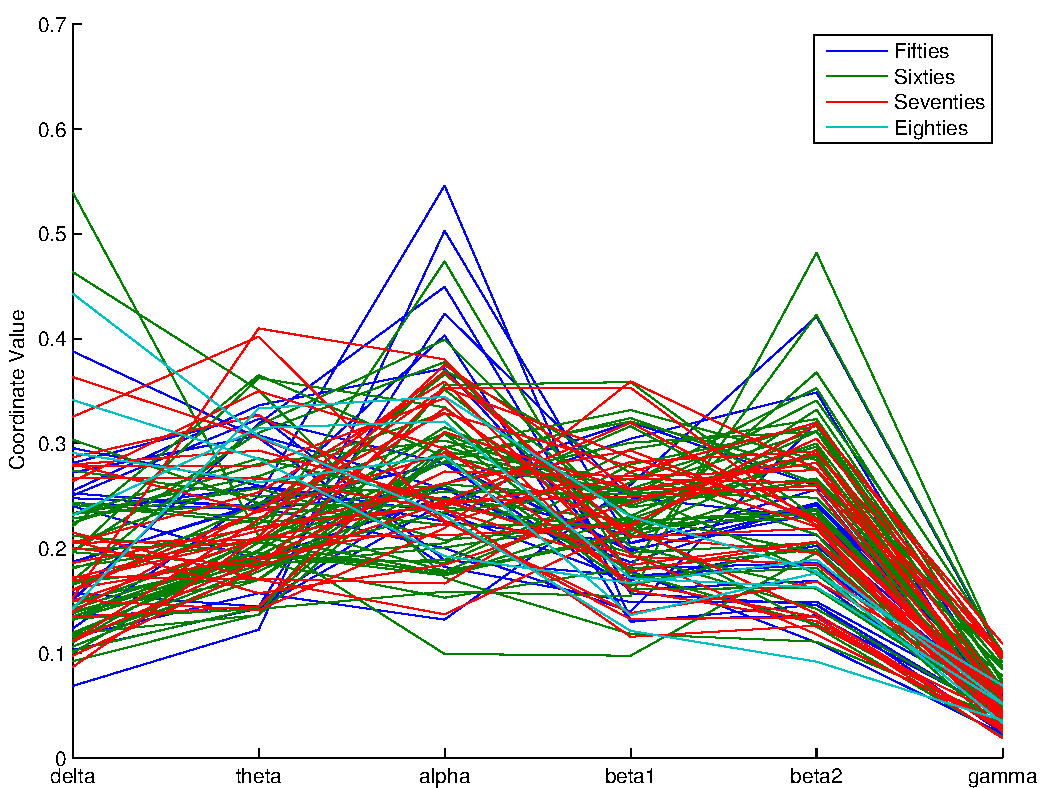
\includegraphics[width=\textwidth]{hparacoords.pdf}
    \caption{The Parallel Coordinate Plot of the healthy dataset divided into different age groups, there is no discernable pattern or separation between them}
    \label{fig:hparacoords}
\end{figure}


\begin{figure}[h!]
  \centering
    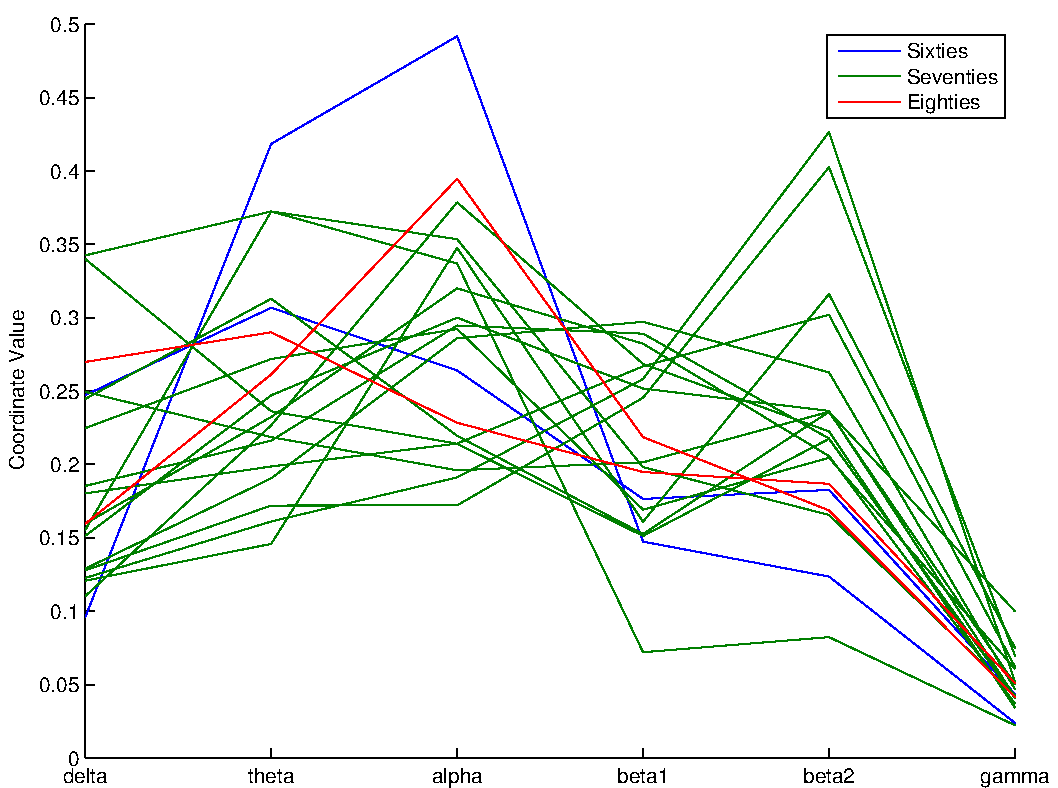
\includegraphics[width=\textwidth]{mciparacoords.pdf}
    \caption{The Parallel Coordinate Plot of the MCI dataset divided into different age groups, there is no discernable pattern or separation between them}
    \label{fig:mciparacoords}
\end{figure}


\begin{figure}[h!]
  \centering
    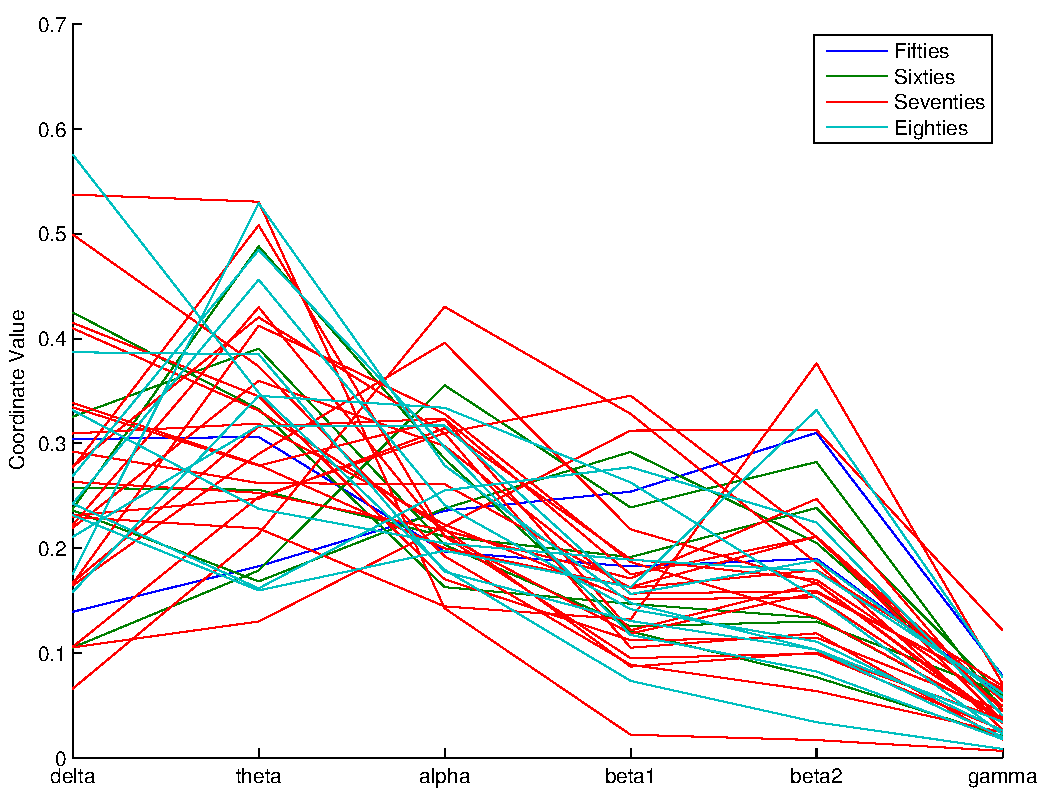
\includegraphics[width=\textwidth]{alzparacoords.pdf}
    \caption{The Parallel Coordinate Plot of the Alzheimer's dataset divided into different age groups, there is no discernable pattern or separation between them}
    \label{fig:alzparacoords}
\end{figure}

As can be seen in Figures \ref{fig:hparacoords}, \ref{fig:mciparacoords} and \ref{fig:alzparacoords} there was no clear distinction between the age groups which further explains why the model for predicting age from the relative powers wasn't very successful and corroborates the results of the t-SNE and PCA projections.


\subsection{Chernoff Faces}

A final and perhaps whimsical method of visualising multidimensional data is the \textit{glyph} based approach of Chernoff faces. These use the values of feature that a sample has to construct a human face, with the feature values being used to determine the size and shape of various parts of the face such as the eyes, mouth etc. The reasoning behind such a visualisation is that the human mind is adept at discerning the differences between human faces and thus can distinguish between relatively similar data more easily when it is presented in this manner. \cite{Chernoff1973}

The Chernoff Faces presented here used the reduced six feature set rather than the full set of 30 features because the Chernoff face package that was used did not have 30 tunable parameters. The features were used to determine the facial characteristics as follows in Table \ref{tab:chernoff}.


\begin{table}[h!]
\begin{center}
\begin{tabular}[h!]{|c|c|}
\hline
Relative Power Band & Chernoff Face Characteristic \\
\hline
Delta & Size of face \\
\hline
Theta & Forehead/jaw relative arc length \\
\hline
Alpha & Shape of forehead\\
\hline
Beta1 & Shape of jaw\\
\hline
Beta2 & Width between eyes\\
\hline
Gamma & Vertical position of eyes\\
\hline
\end{tabular}
\caption{The features and the corresponding facial characteristic in the Chernoff Face}
\label{tab:chernoff}
\end{center}
\end{table}

The datasets for the different classes were separated into the same age groups as before and averaged to produce `composite' Chernoff faces for each age group, note that the MCI dataset had no subjects aged 50-59 and thus it only has faces for the 60-69, 70-79 and 80-89 age groups.


\begin{figure}[h!]
  \centering
    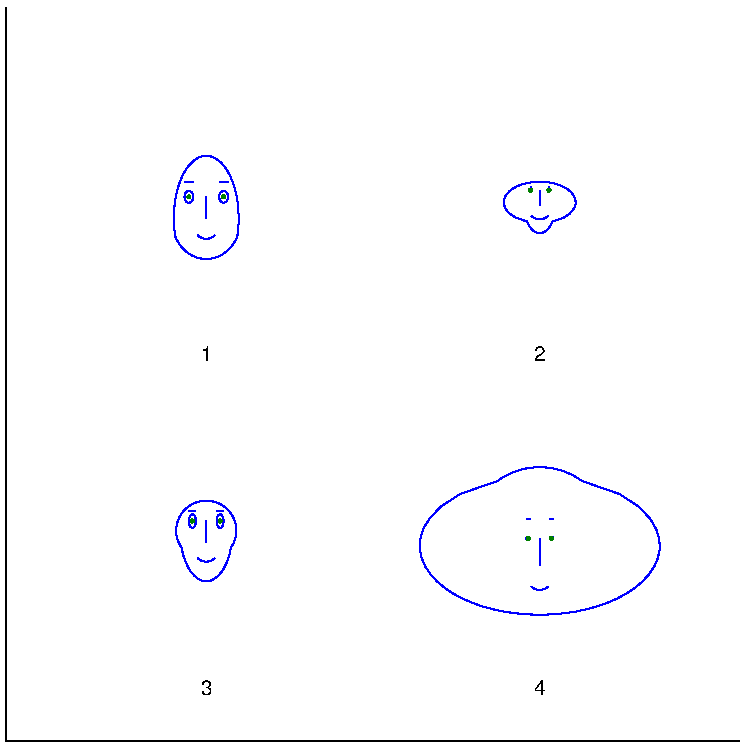
\includegraphics[width=\textwidth]{hChernoffFaces50607080.pdf}
    \caption{The Chernoff faces for the healthy dataset. Face 1 is age group 50-59, Face 2 is age group 60-69, Face 3 is age group 70-79, Face 4 is age group 80-89}
    \label{fig:hchernoff}
\end{figure}

\begin{figure}[h!]
  \centering
    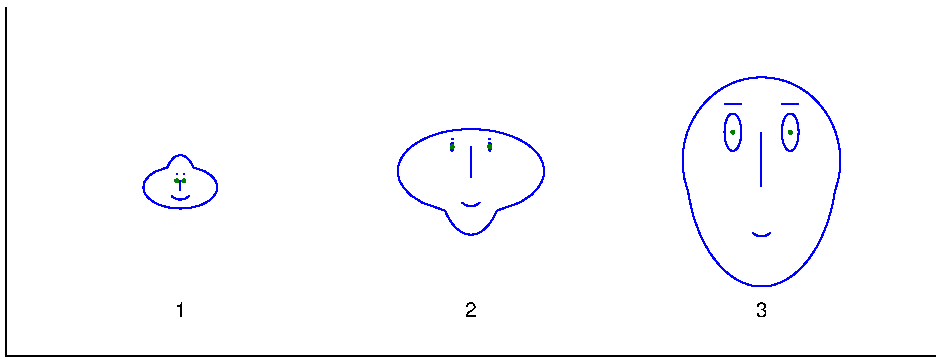
\includegraphics[width=\textwidth]{mciChernoffFaces607080.pdf}
    \caption{The Chernoff faces for the MCI dataset. Face 1 is age group 60-69, Face 2 is age group 70-79, Face 3 is age group 80-89}
    \label{fig:mcichernoff}
\end{figure}

\begin{figure}[h!]
  \centering
    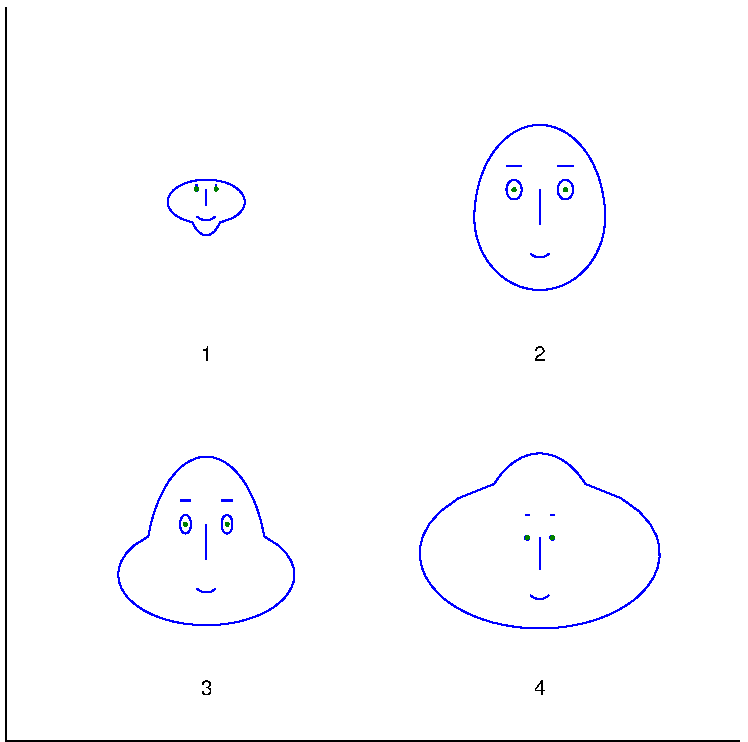
\includegraphics[width=\textwidth]{alzChernoffFaces50607080.pdf}
    \caption{The Chernoff faces for the Alzheimer's Disease dataset. Face 1 is age group 50-59, Face 2 is age group 60-69, Face 3 is age group 70-79, Face 4 is age group 80-89}
    \label{fig:alzchernoff}
\end{figure}

We can observe some differences between the age groups which perhaps explains why the age model didn't completely fail. However, as the relative differences between age groups seem the same in all the classes this implies that distinguishing between them will be very difficult, if possible, which supports the conclusions drawn from the previous visualisation techniques.






\section{Classification}







%deltarp - Size of face
%thetarp - Forehead/jaw relative arc length
%alpharp - Shape of forehead
%beta1rp - Shape of jaw
%beta2rp - Width between eyes
%gammarp - Vertical position of eyes



